%%%%%%%%%%%%%%%%%%%%%%%%%%%%%%%%%%%%%%%%%%%%%%%%%%%%%%%%%%%%%%%%%%%%%%%%%%%
%% This file is part of the book
%%
%% Algorithmic Graph Theory
%% http://code.google.com/p/graph-theory-algorithms-book/
%%
%% Copyright (C) 2009, 2010, 2011 Minh Van Nguyen <nguyenminh2@gmail.com>
%%
%% See the file COPYING for copying conditions.
%%%%%%%%%%%%%%%%%%%%%%%%%%%%%%%%%%%%%%%%%%%%%%%%%%%%%%%%%%%%%%%%%%%%%%%%%%%

\documentclass{article}

\usepackage{tikz}
\usepackage{tkz-berge}  %% for drawing combinatorial graphs
\usetikzlibrary{external}
\tikzexternalize{another-Floyd-Roy-Warshall-demo}

\begin{document}

\begin{figure}
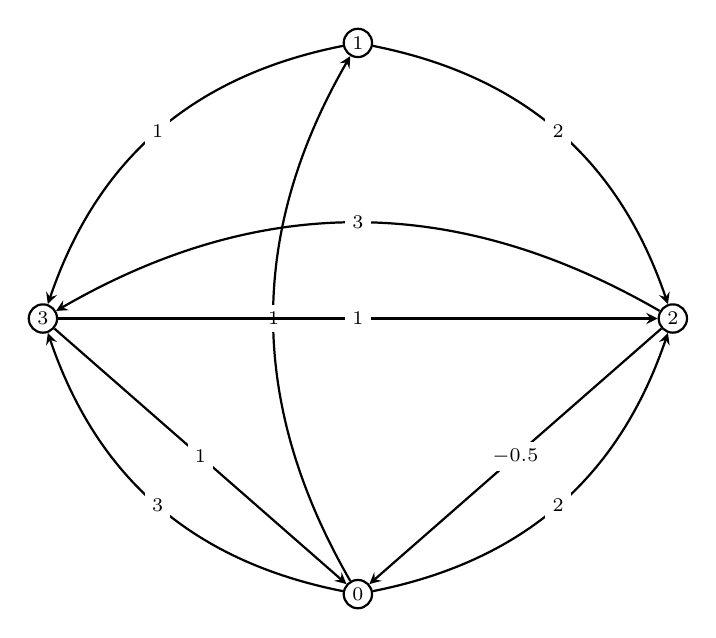
\begin{tikzpicture}
[nodeDecorate/.style={shape=circle,inner sep=1.5pt,draw,thick}]
%% nodes or vertices
\foreach \nodename/\x/\y in {0/0/0, 1/0/7, 2/4/3.5, 3/-4/3.5}
{
  \node (\nodename) at (\x,\y) [nodeDecorate] {\scriptsize$\nodename$};
}
%% edges or lines
\tikzstyle{EdgeStyle}=[->,>=stealth,thick]
\tikzstyle{LabelStyle}=[fill=white]
\foreach \startnode/\endnode/\bend/\weight in {
  0/1/bend left/1, 0/2/bend right/2, 0/3/bend left/3,
  1/2/bend left/2, 1/3/bend right/1, 2/0/bend left=0/-0.5,
  2/3/bend right/3, 3/0/bend left=0/1, 3/2/bend left=0/1}
{
  \scriptsize
  \Edge[label=$\weight$,style=\bend](\startnode)(\endnode)
}
\end{tikzpicture}
\end{figure}

\end{document}
